\documentclass{standalone}
\usepackage{tikz}
\usetikzlibrary{shapes.geometric, arrows.meta, positioning}

% Define flowchart styles
\tikzstyle{startstop} = [ellipse, rounded corners, minimum height=1.5em, minimum width=3em, draw=black, fill=red!20, text centered, font=\footnotesize]
\tikzstyle{inputoutput} = [trapezium, trapezium left angle=70, trapezium right angle=110, minimum height=1.5em, draw=black, fill=blue!20, text centered, font=\footnotesize]
\tikzstyle{process} = [rectangle, minimum height=1.5em, minimum width=3em, draw=black, fill=green!20, text centered, font=\footnotesize]
\tikzstyle{decision} = [diamond, minimum height=1.5em, minimum width=3em, draw=black, fill=yellow!20, text centered, font=\footnotesize]
\tikzstyle{arrow} = [thick,->,>=stealth]

\begin{document}

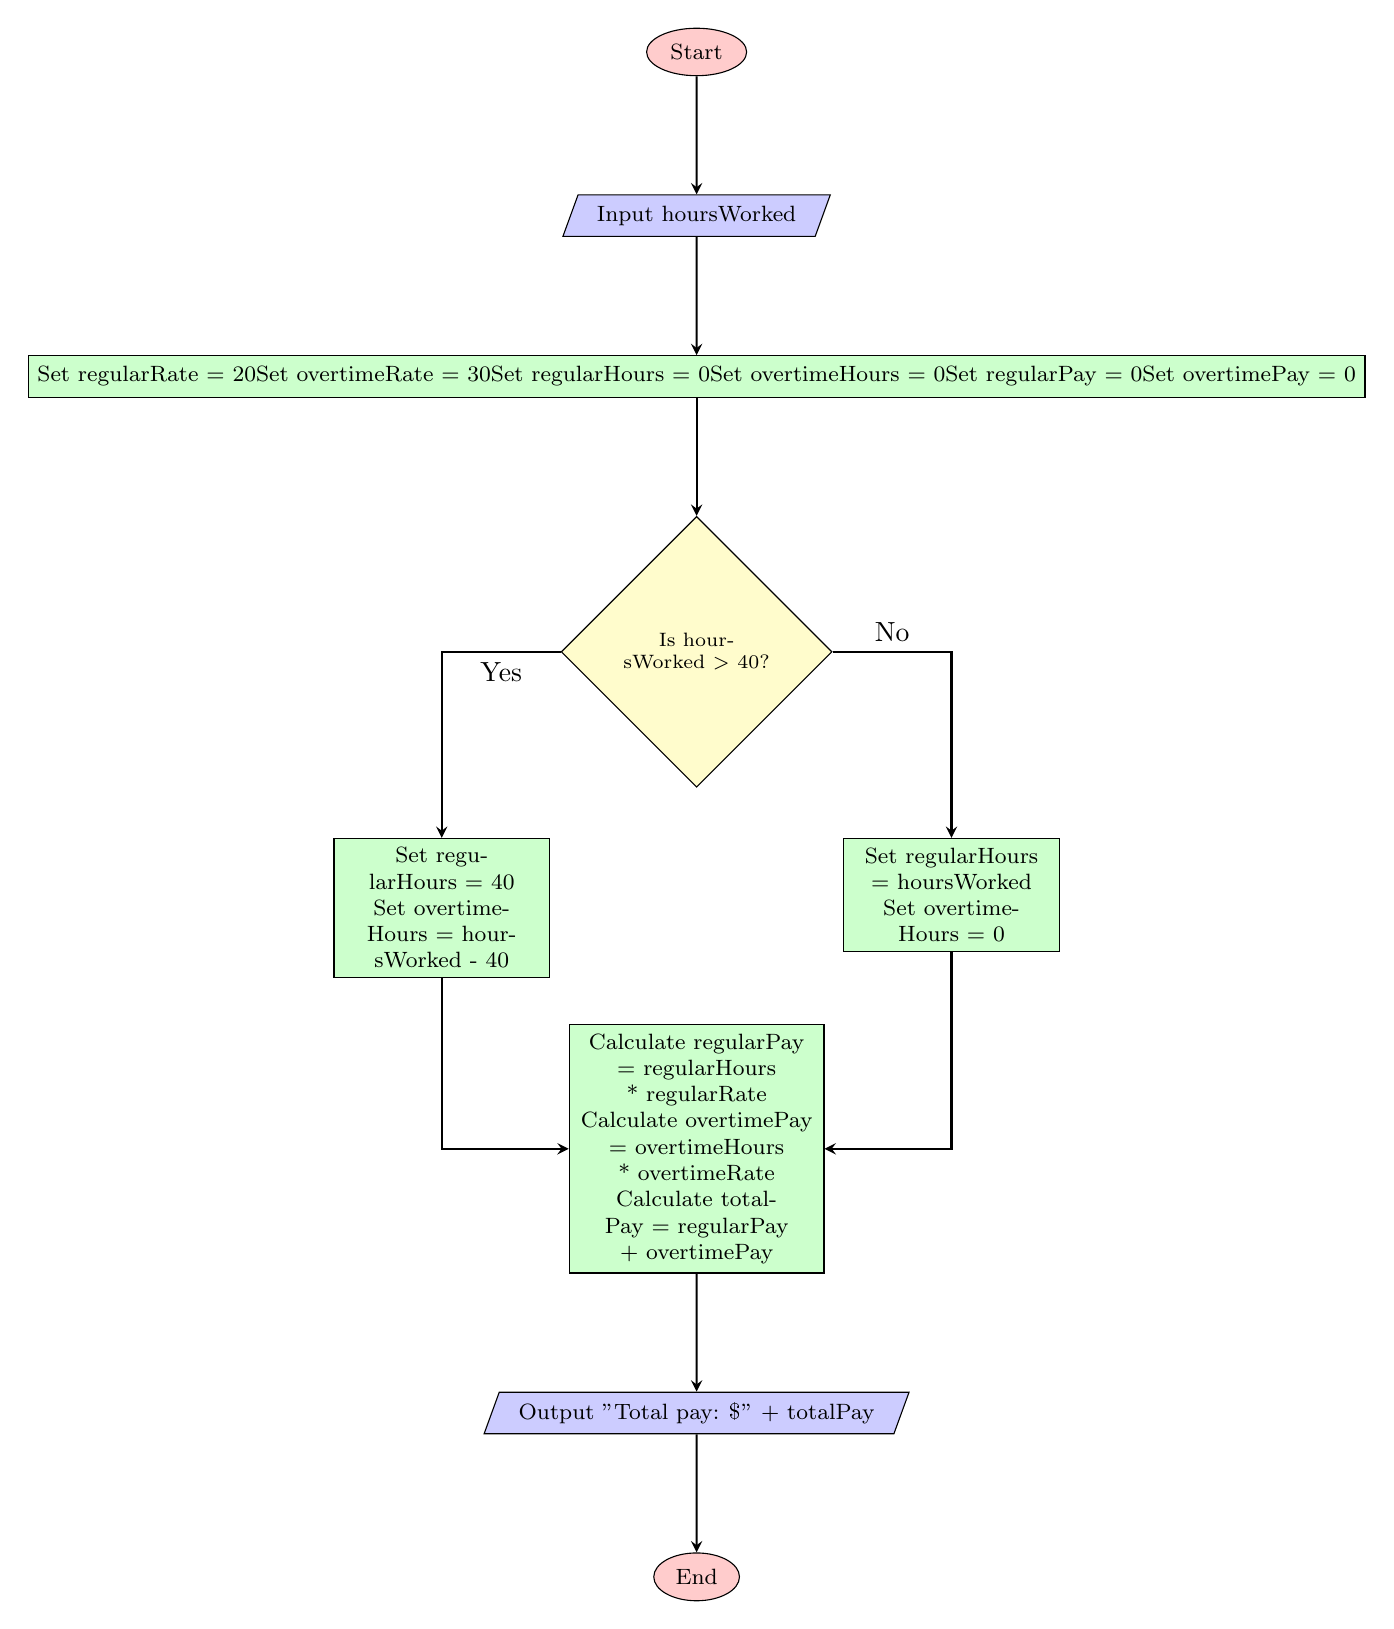
\begin{tikzpicture}[node distance=1.5cm and 1cm, auto]

% Nodes
\node[startstop] (start) {Start};
\node[inputoutput, below=of start] (input) {Input hoursWorked};
\node[process, below=of input] (init) {Set regularRate = 20\\Set overtimeRate = 30\\Set regularHours = 0\\Set overtimeHours = 0\\Set regularPay = 0\\Set overtimePay = 0};
%\node[decision, below=of init, text width=2.5cm] (decision) {Is hoursWorked > 40?};
\node[decision, below=of init, text width=2.5cm, font=\scriptsize] (decision) {Is hoursWorked $>$ 40?};
\node[process, below left=of decision, text width=2.5cm] (yes) {Set regularHours = 40\\Set overtimeHours = hoursWorked - 40};
\node[process, below right=of decision, text width=2.5cm] (no) {Set regularHours = hoursWorked\\Set overtimeHours = 0};
\node[process, below=of decision, yshift=-1.5cm, text width=3cm] (calc) {Calculate regularPay = regularHours * regularRate\\Calculate overtimePay = overtimeHours * overtimeRate\\Calculate totalPay = regularPay + overtimePay};
\node[inputoutput, below=of calc] (output) {Output "Total pay: \$" + totalPay};
\node[startstop, below=of output] (end) {End};

% Arrows
\draw[arrow] (start) -- (input);
\draw[arrow] (input) -- (init);
\draw[arrow] (init) -- (decision);
\draw[arrow] (decision) -| node[near start] {Yes} (yes);
\draw[arrow] (decision) -| node[near start] {No} (no);
\draw[arrow] (yes) |- (calc);
\draw[arrow] (no) |- (calc);
\draw[arrow] (calc) -- (output);
\draw[arrow] (output) -- (end);

\end{tikzpicture}

\end{document}